\documentclass[12pt, oneside]{article}   	% use "amsart" instead of "article" for AMSLaTeX format
\usepackage{geometry}                		% See geometry.pdf to learn the layout options. There are lots.
\geometry{letterpaper}                   		% ... or a4paper or a5paper or ... 
\geometry{legalpaper, portrait, margin=1in}
\usepackage[parfill]{parskip}    			% Activate to begin paragraphs with an empty line rather than an indent
\usepackage{graphicx}				% Use pdf, png, jpg, or eps§ with pdflatex; use eps in DVI mode
\usepackage{amssymb}
\usepackage{multicol}
\usepackage{abstract} 
\usepackage{graphicx}
\usepackage{caption}

\title{Saito: A Big-Data Blockchain with Proof-of-Transactions}
\author{David Lancashire}
\date{January 1, 2018}	

\begin{document}
\maketitle

%\section{}
%\subsection{}



\begin{onecolabstract}
Saito is a blockchain designed to process terabytes of data every day, a level of scalability it achieves by coupling a transient ledger to a proof-of-transactions mechanism that pays explicitly for the bandwidth used by the network. Saito evolves towards an optimal network structure while eliminating sibyl-attacks, fee-recycling attacks, block-withholding attacks and more. It provides a decentralized and efficient network platform on which to build bandwidth-intensive Internet applications like email, social networks, cryptocurrency payment channels, and much more.
\end{onecolabstract}


\begin{multicols}{2}
Saito is a cryptocurrency designed for applications that need to send large amounts of data across the Internet. It can be used to build decentralized versions of most Google services, along with un-astroturfable Internet forums, social networks, pay-to-play websites, distributed key registries that are secure from MITM attacks, payment channels, and much more.

More generally, Saito is a complete solution to the question of how to build a terabyte-level network. And what is meant by this is simple: the point is that a Saito-class blockchain can scale to the point underlying network hardware imposes physical limits on the speed of data transfer in the network. We believe the practical limit for a Saito blockchain today is in the order of 100 TB of data per day, and that we will reach petabyte level blockchain within a decade.

If you are interested in the technical design of the Saito network, please skip to section. In the next section we describe why these steps are necessary by explaining the underlying problems with existing blockchain designs (and their solutions). If you wish to jump to the details of the Saito implementation, please skip to Section III.


1. THE PROBLEM

One of the reasons that the blockchain scaling debate has been so problematic is that few people understand the real issues, which are 

Specifically.


But what causes this? In 

* identify nodes performing useful work in the routing network
* separate the coinbase from blocks so that block producers cannot game the token-issuing mechanism
*

In his writings on Bitcoin, Craig Wright has argued that . This is correct, and it poses no problems in , but it causes problems at scale. The reason for this is that markets are imperfect and the incentive mechanisms in Bitcoin suffer from problems that 





In the Saito network we make two changes to enable terabyte-level scaling. The first is embracing a "transient blockchain" and the second is the use of a novel consensus mechanism that we call proof-of-transactions. 

1. THE TRANSIENT BLOCKCHAIN

The principle behind the transient blockchain is simple: allow the nodes in the network to delete the oldest blocks in the ledger at predictable intervals ("genesis periods"). The length of the genesis period can be set dynamically if needed. At the extreme of a blockchain designed to handle global email traffic, the genesis period may be as short as 24 hours.

As such, the transient blockchain can be considered a form of pruning where the UTXO slips added to new blocks simply become unspendable after a certain period of time, with the limit enforced by the consensus rules of the blockchain so that blocks containing invalid transactions are themselves deemed invalid. Core nodes in the routing network are no longer required to maintain a permanent ledger and it is possible to accurately predict the true cost of transaction storage. Network operating costs also remain stable as old transactions are removed at roughly the same rate that new transactions are added.\footnote[1]{The most resilient parasite in the blockchain community is the rarely-challenged notion that blockchains require permanent ledgers. Yet this is entirely false -- the purpose of a consensus mechanism is to allow the network to reach consensus about which tokens being *added* to the network have value and ensure that value persists for long enough that they can be exchanged for other resources needed to run the network. None of this requires tokens to have value in perpetuity.}

Under this system, the burden of archiving the network history passes -- as it does in the consumer Internet -- from the routing nodes in the network to the servers and users that actually care about the data. And in cases where it is desirable for data to remain on-chain, it can simply be rebroadcast to the front of the chain with the appropriate fee to cover the next genesis period. The automatic rebroadcasting of expiring slips can even be enabled, if desired, through the consensus rules of the blockchain.

The security trade-off in this approach is that new nodes joining the network become vulnerable to attack at their point of initial connection. And yet this is nothing new to Saito, as the security that syncing from the genesis block offers is largely illusory. How many Bitcoin users check that their software is syncing from the correct hash? And how can they be sure the software is using that hash? The reality is that security in software packaging and deployment cannot be reduced to a hash, and we must get rid of the illusion that it can to create a truly secure and decentralized Internet.

While this avoids the problem of the blockchain growing too large for network nodes to store, and ensures space on the blockchain can be priced accurately even as storage times approach infinity, this change does not pay for the bandwidth needed by nodes in the peer-to-peer network. To solve this second problem we requires a new security method we call proof-of-transactions:

2. PROOF-OF-TRANSACTIONS

Under proof-of-transactions, any node can create a block at any time provided it pays a "burn fee" set by the network as the cost of doing so. This burn fee is set to a high value immediately after a block is found and decreases gradually until it hits zero. Since nodes will issue blocks as soon as it becomes profitable for them to do so, our pace of block production is determined by the overall volume of transactions in the network.

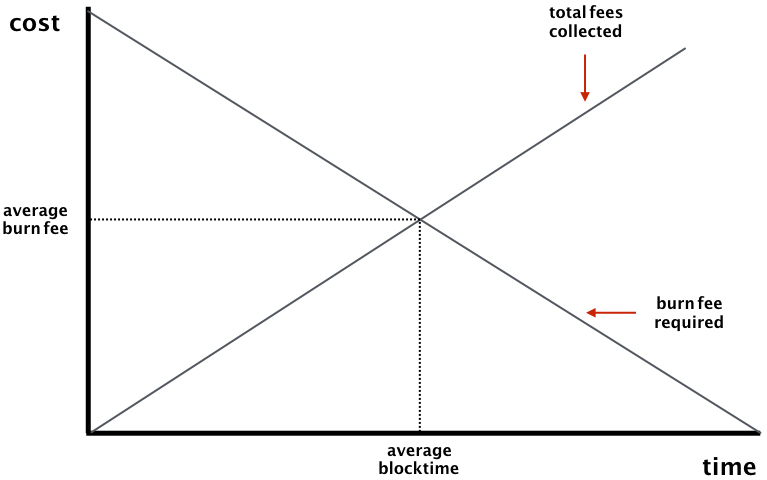
\includegraphics[width=.45\textwidth]{saito2.jpeg}

Our burn fee makes attacking the network expensive, since any increase in the pace of block production requires attackers to pay more in transaction fees than the network is actually collecting. In practice, this means attackers must burn their own capital to attack the network by creating fake transactions that include real fees. It can be easily seen from Figure 2 that it is impossible for attackers to produce blocks at a faster pace than the main chain without taking this step.

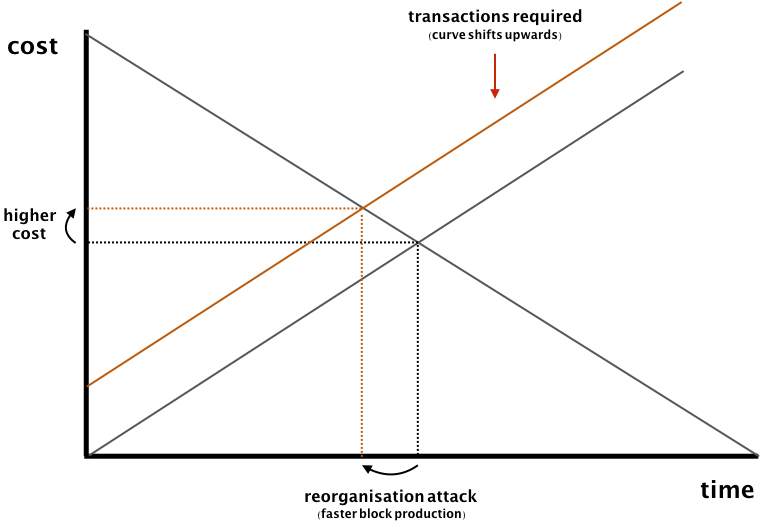
\includegraphics[width=.45\textwidth]{saito3.jpeg}

For reasons that are outlined in Section 4, Saito forces attackers to pay the entire burn fee rather than just cover the marginal difference over the main chain. We also increase the cost of attacks over time by adjusting our burn fee upward to keep blocktime constant as transaction volume grows. This allows the network to offer comparable security to Bitcoin in the sense that the cost of a chain-reorganization attack can always be quantified, and users and applications that require significant guarantees against non-reversibility can calculate the cost of a reorganization attack and wait for the appropriate number of confirmations needed to make chain reorganizations improbable.

There is a major problem with this approach however, which lies in the economic consequences of requiring nodes to burn capital to produce blocks:

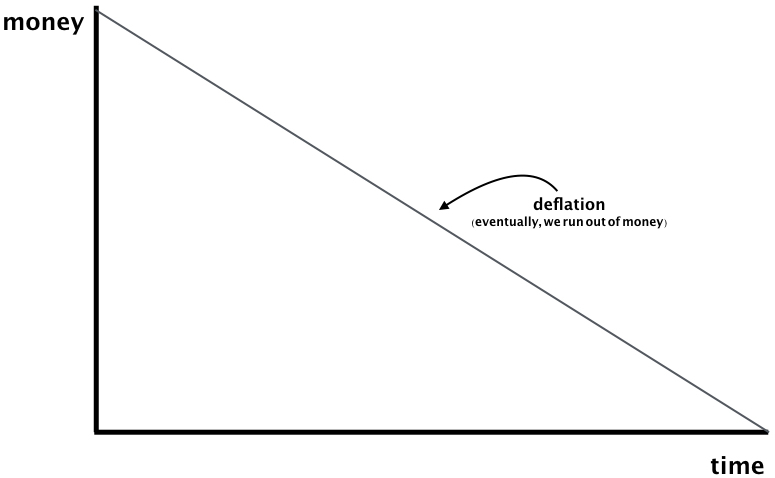
\includegraphics[width=.45\textwidth]{saito4.jpeg}

Avoiding a deflationary crash requires us to inject tokens into our network to keep it from collapsing. But how? The bitcoin solution of attaching the coinbase directly to blocks would eliminate the entire point of having a burn fee -- what is the point of spending money to produce a block if one gets it all back immediately? And where else can the network insert funds? As long as block-producing nodes have any influence over how funds are allocated a savvy attacker can sibyl the network for profit, earning profits less by processing transactions and more by gaming the token-issuing mechanism.

Fortunately, there is a solution to this problem, which involves the recycling of the burn fee back into the network through a process that cannot be coopted by any of the players in the network. We achieve this through a zero-sum competition between bandwidth-expending nodes and CPU-expending miners in the network. We call this battle for the "paysplit" of the network.

3. PAYSPLIT

Whenever a node produces a block, it collects what profit it can and bundles all remaining fees into a "golden ticket" that contains (1) a computational puzzle for miners to solve, and (2) a vote to increase, decrease, or hold constant the "paysplit" of the network (the percentage of all golden tickets that are paid out to miners). These tickets are included (by default) in all blocks produced. Miners listening on the network then choose which blocks to solve and -- should they find a solution to the cryptographic puzzle -- propagate their solution back into the network as a regular fee-paying transaction. In addition to a proof-of-solution, these miner transactions also include a separate vote on whether to increase, decrease, or hold constant the difficulty of the computational puzzle.

The golden ticket system can be visualized as follows:

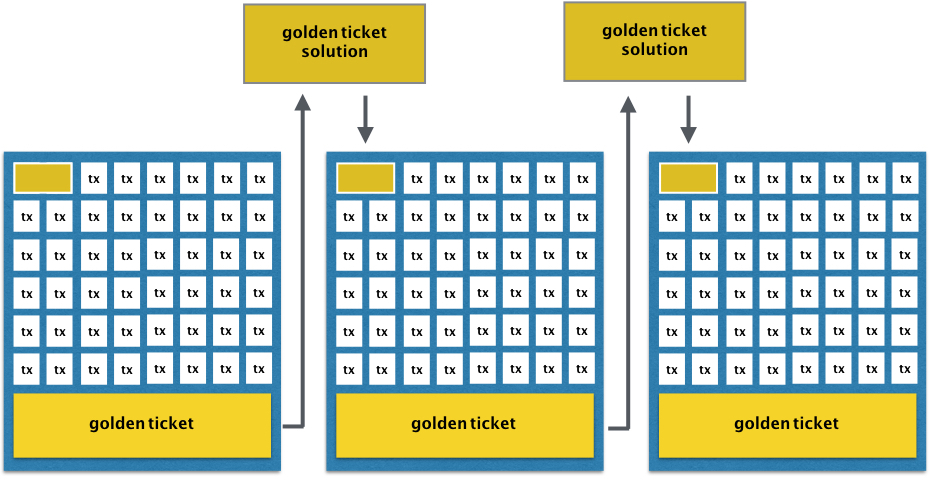
\includegraphics[width=.45\textwidth]{saito7.jpeg}

In order to increase the security of the blockchain, we specify that only one solution may be provided for any golden ticket, and that solution must be included in the very next block. If these conditions are met, our two votes take effect, and the funds locked into the golden ticket are released to the network, split between the miner that found the solution and a random node in the peer-to-peer network. And in the event a "golden ticket" is not solved? The funds locked away will eventually fall off the transient blockchain, at which point they can be recycled back into our economy in the coinbase of another golden ticket. 

This game is counterintuitive to most bitcoiners because it separates the act of "producing blocks" from the act of "issuing tokens". Also because all actors are trapped in a delicate dance requiring collusion and cooperation alike. For while both nodes and miners want at least one solution per golden ticket (because otherwise no-one gets paid), their interests otherwise diverge: miners prefer a high paysplit and high difficulty level, while nodes prefer a low paysplit and low difficulty level. Given that votes must pass between both players to change consensus settings, we end up with a competitive dynamic where agents in both groups are constantly trading-off their individual short-term against their collective long-term interests.

There are many obvious variants, such as the replacement of a mining puzzle with a proof-of-stake variant. The key observation is that full-nodes that have miner support will produce blocks at a faster rate and be more profitable than those who do not. And miners who have the support of full-nodes will also be more profitable. This creates a dynamic where excessive profits in any sector of the network (i.e. bandwidth provision) will attract competition that will support out-group actors in order to earn immediate supra-market profits. It is impossible without locking down the open access of the network, which is possible in other blockchains and guaranteed here by the fact that routing is incentivized.

This economic design makes the Saito Network robust and pushes us towards an equilibrium point at which the security provided is optimal for both nodes and miners given their relative ease of collusion and defection, something that is itself determined by the market structure surrounding the economics of bandwidth and security provision. A useful thought experiment is exploring how the security of this two-player system degrades to offer only bitcoin-level security as the paysplit approaches extreme values.

Since we acknowledge that this level is arbitrary and may not reflect the needs of the applications on the network, we allow users on the network to tag their transactions with an optimal paysplit vote. Should a user-originated transaction contain such a vote, our system insists that it can only be included in a block which votes in the same direction. Users who choose to take sides in the ongoing struggle between nodes and miners thus sacrifice the reliability and speed of transaction confirmation, but gain marginal influence over how the network allocates fees.

4. ADDITIONAL SECURITY

Saito takes additional steps to secure the network. In order to deter sibylling, we have nodes sign transactions as they propagate through the network, adding to each an unforgeable history of the path it takes from its point of origin to its point of confirmation. We also decrease the amount of each transaction fee that nodes can allocate to paying their burn fee with each hop a transaction takes along the network, and specify that nodes cannot use any fees for that purpose from transactions that do not include them in their transaction path. In order to ensure that nodes cannot influence the distribution of funds from the golden ticket, we also specify that the node in the peer-to-peer network which wins the node share of the golden ticket is selected using a random variable sourced from the miner solution, with the winner selected from the pool of nodes contained in the transaction propagation paths found in the previous block.

These additional restrictions secure our network from common attacks in other cryptosystems which -- oddly -- are not commonly recognized as attacks. In Saito, for instance, transactions are naturally valuable to nodes which participate in the P2P network and useless to attackers who lurk on the edges. Fee-sourcing attacks and transaction theft are also impossible: the fact that nodes must participate in the P2P network to harvest transactions defends us against subtle attacks like those posed by the bitcoin FIBRE network, a closed-access network which benefits its participants by undermining the profitability of nodes which support the peer-to-peer network. And sibylling becomes an unprofitable strategy because it necessarily adds hops in transaction routes, making sibyls visible to other nodes and providing an evolutionary mechanism whereby weaker nodes which permit themselves to be sibylled necessarily lose revenue over time. 

And hoarding? Even hoarding is minimized because nodes that merely participate in transaction routing have a chance of winning the golden ticket reward. Over the mid-term, Saito rewards lite-nodes in proportion to their work as much as it does core network nodes.

Security is also reinforced by the competitive economic structure of our game in fascinating ways. Note that if network security falls too low, the network is incentivized to increase it by voting to pay miners more. How this secures the network is not obvious, but it does: greater pay for miners increases the amount needed to attack the network. A higher paysplit also supports the threatened chain in the long-run, and speeds up block-issurance as miners compete to have their solutions included over those of their peers. Even in situations where the network is not under active attack, the miner/node battle over the paysplit vote also serves a defensive "canary in the coalmine" function, encouraging miners to issue their own pro-miner blocks if they control enough hashpower to support the block.

5. SUMMARY

Saito corrects the underlying economic problems that are preventing other blockchains from scaling. In the process of doing so, it introduces at least six major innovations in blockchain design: the transient blockchain, the burn fee, the usable transaction fee that quantifies the value of routing paths, the golden ticket system, the multi-party voting mechanism, and the chain of cryptographic signatures we embed in transactions that permits our network to identify and reward productive nodes without the need to maintain an objective view of network topology.  

We have secured provisional patent protection for these innovations and welcome contact from other blockchain projects looking to incorporate one or several of these innovations in their own networks, ideally through the creation of a defensive patent alliance and sharing resources needed to tackle genuinely big-data problems in the blockchain space.

More information about how the Saito blockchain works can be found on our website (http://saito.tech) along with a working demo of the network and instructions on how to get started building applications *today*. We welcome contact from developers looking to build the next generation of the Internet and will help get you up to speed.



\end{multicols}
 
\end{document}
